\chapter{\textbf{Конструкторский раздел}}

\hfill

Можно разбить задачу проектирования микросервиса на подзадачи:
\begin{itemize}
\item описание функциональности и поведения;
\item выделение сущностей предметной области;
\item разработка структуры БД;
\item проектирование компонентов микросервиса.
\end{itemize}

В данном раздел рассматривается структура микросервиса мессенджера, каждого из его компонентов. 

\section{\textbf{Функциональная модель}}

\hfill

На рисунке \ref{img:idef0} изображена функциональная модель, отобра­жающая структуру и функции системы.

\begin{figure}[H]
	\centering
	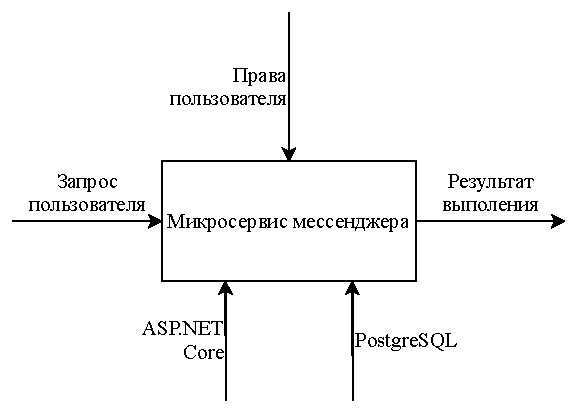
\includegraphics[scale=1]{idef0}
	\caption{Функциональная модель микросервиса мессенджера. }
	\label{img:idef0}
\end{figure}

\section{\textbf{Сценарий использования}}

\hfill

В данном разделе необходимо построить Use Case Diagram (диаграмму прецедентов). Она состоит из графической диаграммы, описывающей действующие лица и прецеденты -- конкретные действия, которые выполняет пользователь при работе с системой. 

Данная диаграмма предназначена для определения функциональных требований, действующие лица не будут делится по ролям и правам, так как за это отвечает внешняя система. 

На рисунке \ref{img:usechat} представлена Use Case диаграмма для действий с чатами. 

\begin{figure}[H]
	\centering
	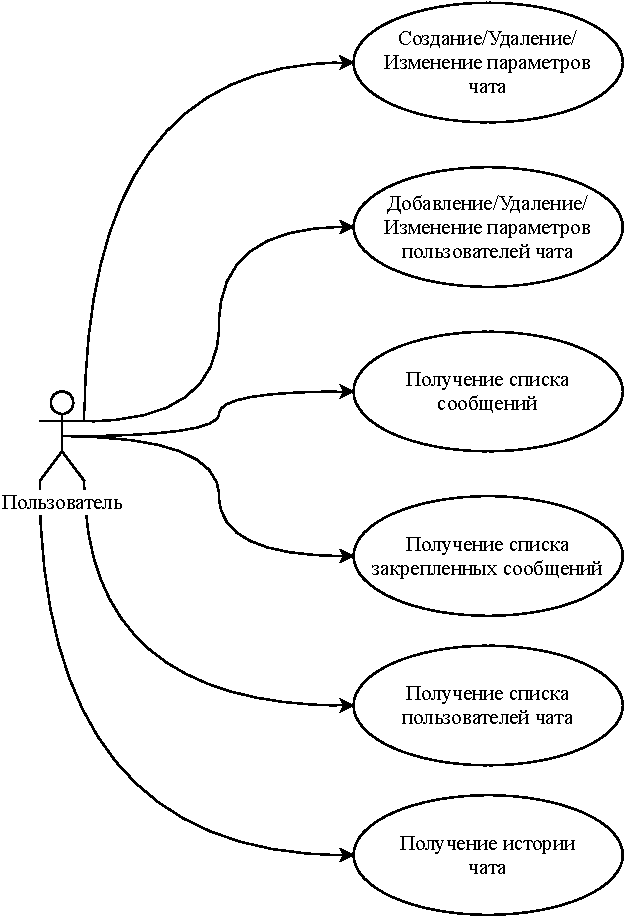
\includegraphics[scale=1]{usechat}
	\caption{Use Case диаграмма для действий с чатами. }
	\label{img:usechat}
\end{figure}

На рисунке \ref{img:useuser} представлена Use Case диаграмма для действий с пользователями. 

\begin{figure}[H]
	\centering
	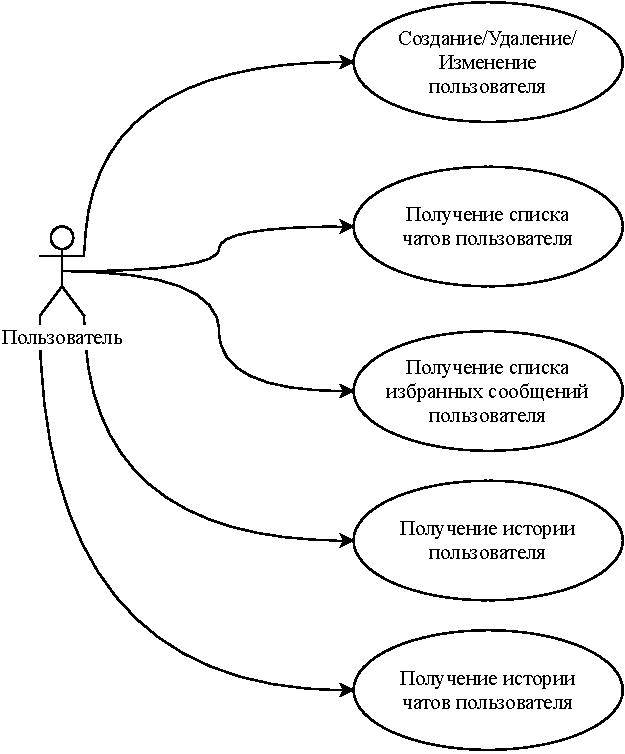
\includegraphics[scale=1]{useuser}
	\caption{Use Case диаграмма для действий с пользователями. }
	\label{img:useuser}
\end{figure}

На рисунке \ref{img:usemessage} представлена Use Case диаграмма для действий с сообщениями. 

\begin{figure}[H]
	\centering
	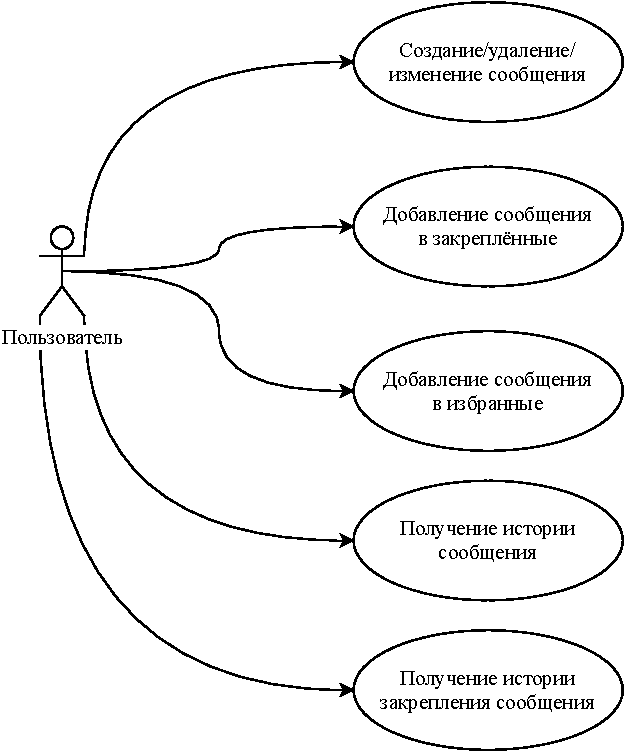
\includegraphics[scale=1]{usemessage}
	\caption{Use Case диаграмма для действий с сообщениями. }
	\label{img:usemessage}
\end{figure}


\section{\textbf{База данных}}

\hfill

Далее были выделены сущности предметной области и построена ER-диаграмма, которая содержит 14 таблиц. Диаграмма представлена на рисунке \ref{img:er}. Таблица \ref{table:database} содержит описание сущностей базы данных. 

\begin{figure}[H]
	\centering
	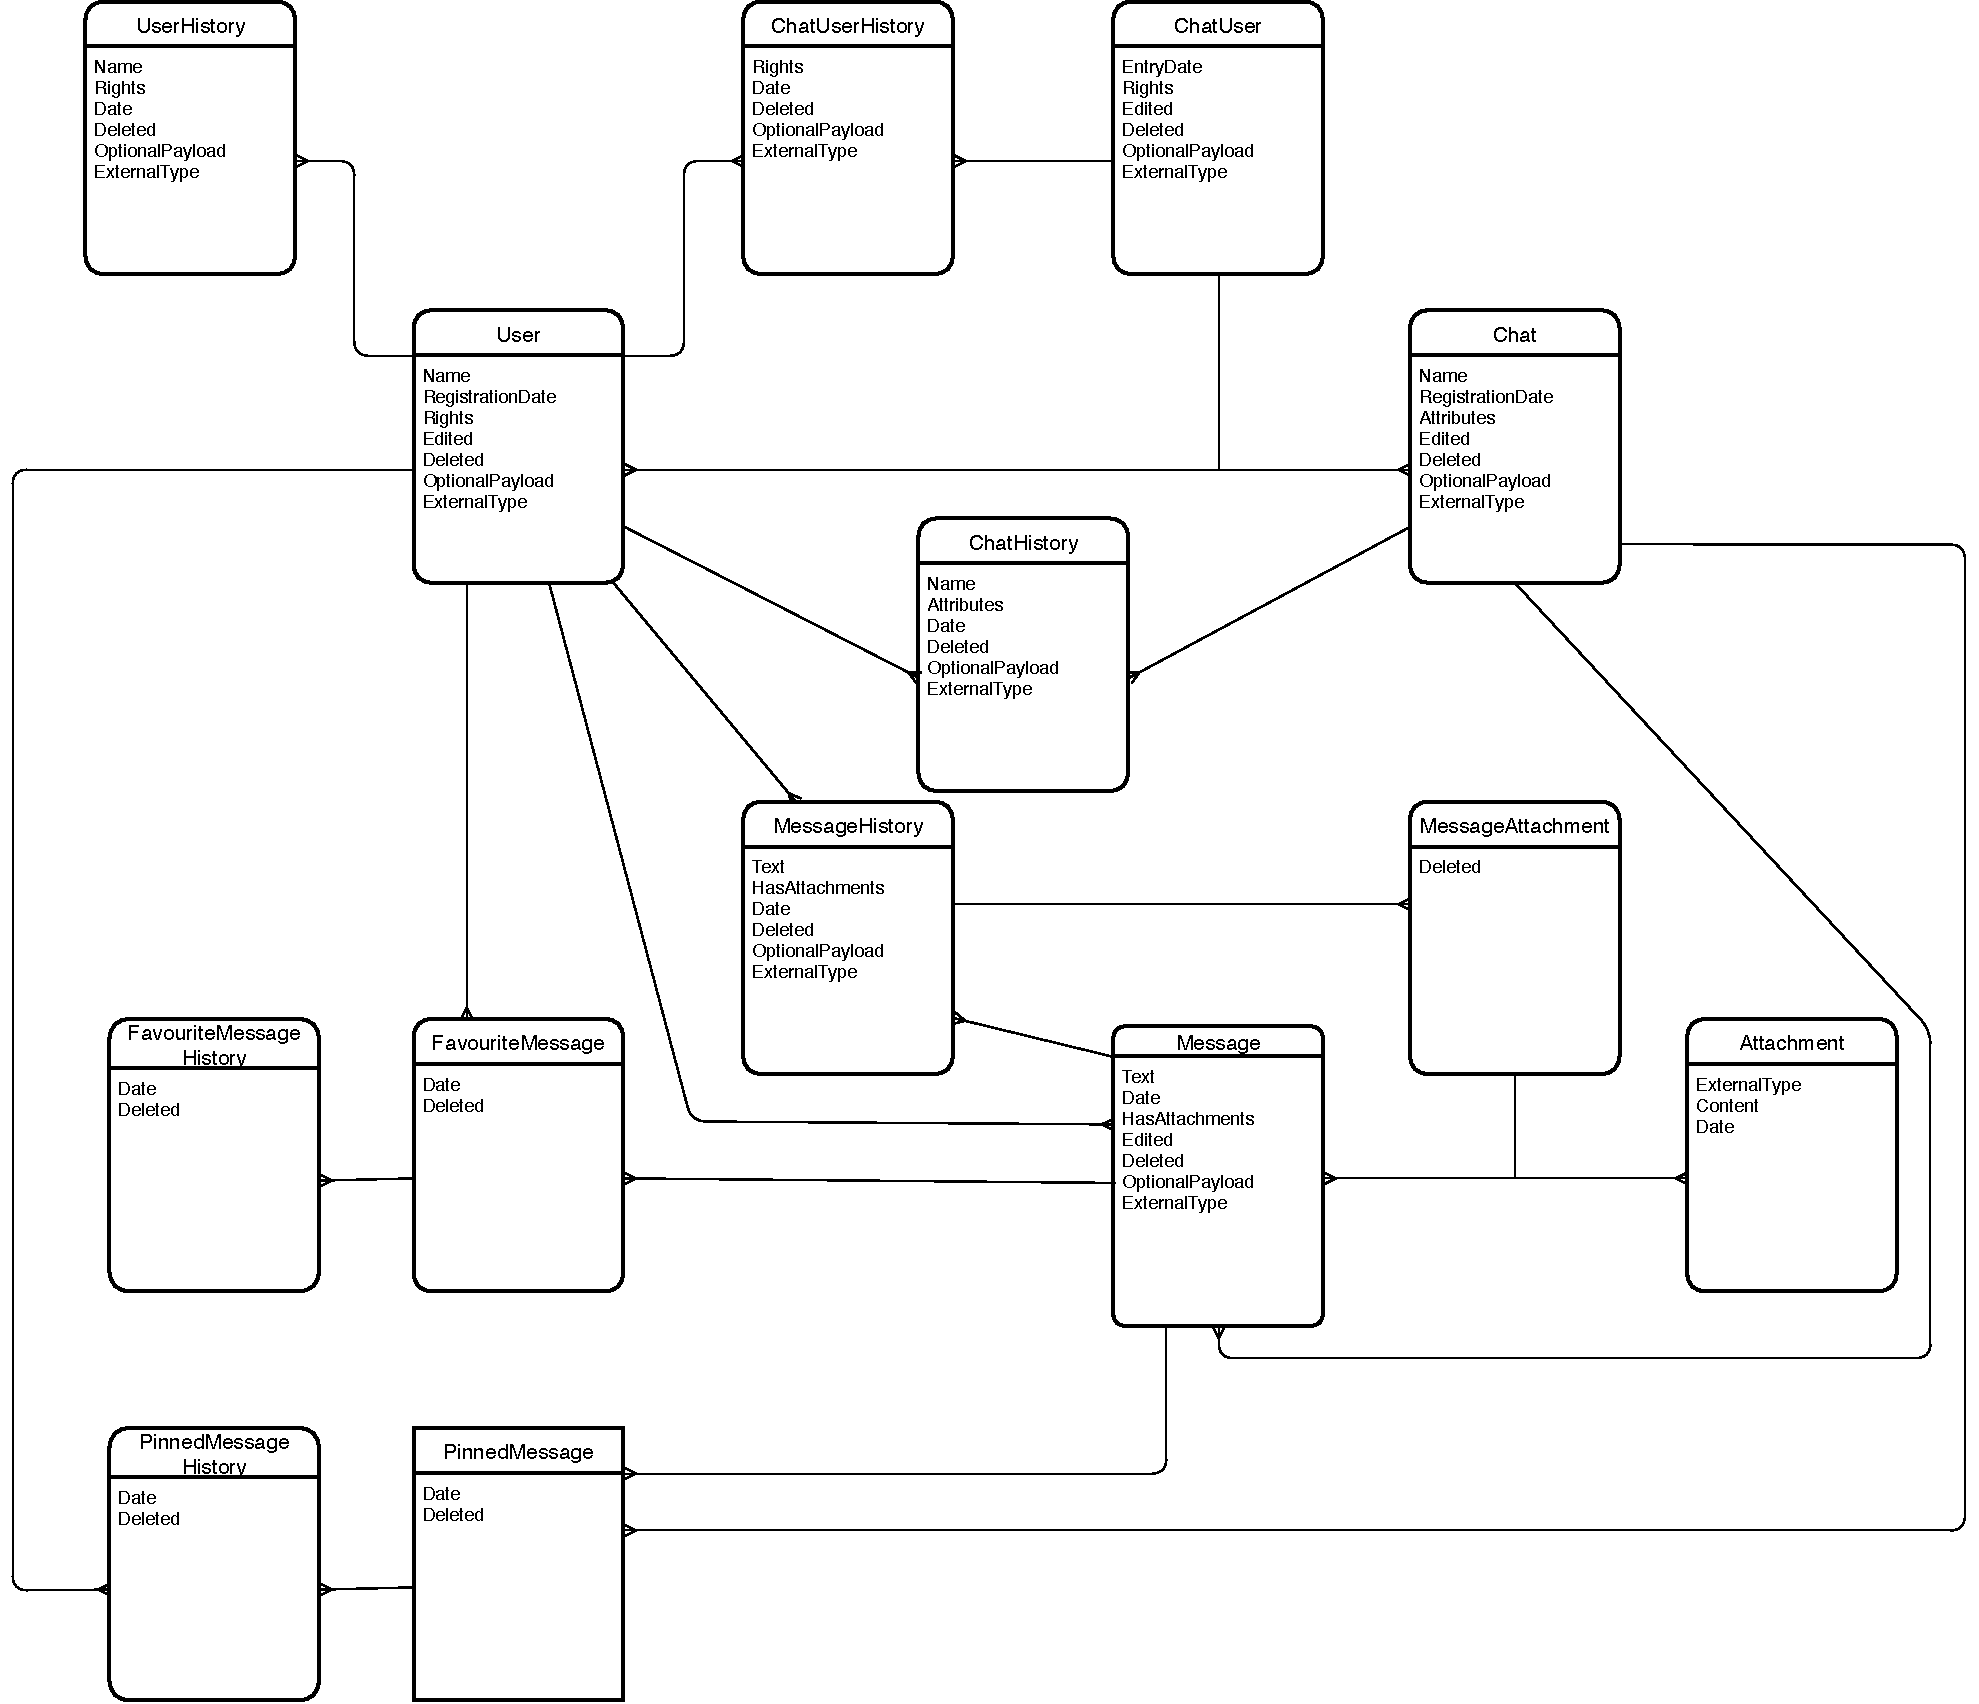
\includegraphics[scale=0.53]{er}
	\caption{ER-диаграмма базы данных. }
	\label{img:er}
\end{figure}

\begin{table}[H]
\caption{Описание сущностей базы данных. }
\begin{tabular}{|p{4cm}|p{12cm}|}
\hline
Название таблицы&Описание \\ \hline
User & Пользователи \\ \hline
UserHistory & История изменений пользователей \\ \hline
Chat & Чаты \\ \hline
ChatHistory & История изменений чатов \\ \hline
ChatUser & Пользователи чатов (соединительная таблица между пользователями и чатами) \\ \hline
ChatUserHistory & История изменений пользователей чата \\ \hline
Message & Сообщения \\ \hline
MessageHistory & История изменений сообщений \\ \hline
Attachment & Вложения \\ \hline
MessageAttachment & Вложения сообщений (соединительная таблица между вложениями и сообщениями)  \\ \hline
FavouriteMessage & Избранные сообщения пользователя \\ \hline
FavouriteMessage History & История изменений избранных сообщений пользователя \\ \hline
PinnedMessage & Закрепленные сообщения в чатах \\ \hline
PinnedMessage History & История изменений закрепленных сообщений в чатах \\ \hline
\end{tabular}
\label{table:database}
\end{table}

\section{\textbf{Проектирование архитектуры}}

\hfill

Необходимо спроектировать абстрактный микросервис мессенджера. На рисунке \ref{img:components} представлена диаграмма компонентов микросервиса. 

\begin{figure}[H]
	\centering
	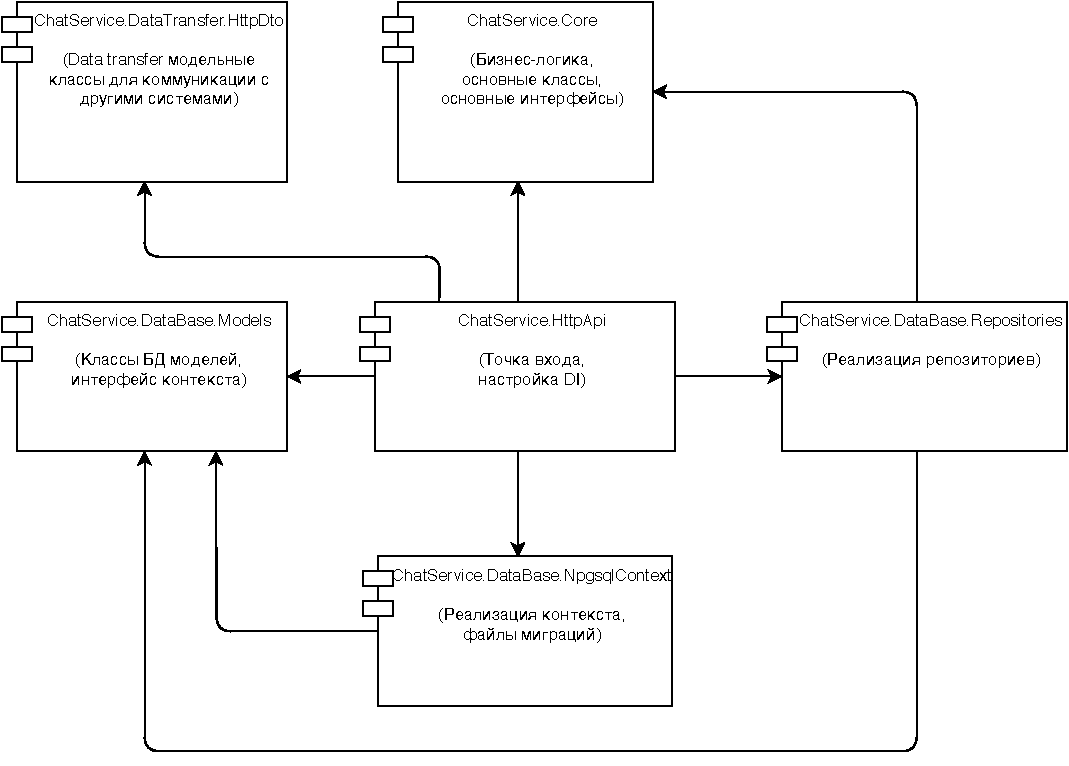
\includegraphics[scale=0.95]{components}
	\caption{Диаграмма компонентов микросервиса. }
	\label{img:components}
\end{figure}

\begin{enumerate}
\item[1. ] \textbf{ChatService.HttpApi}

ChatService.HttpApi -- точка входа в проект, инициализирует и конфигурирует IoC контейнер, здесь происходит настройка DI. 

Смысл IoC (Inversion of Control/инверсия управления) заключается в том, что модули верхнего уровня не должны зависеть от реализации модулей нижнего уровня \cite{solid}. То есть, например, компонент в приложении, который отвечает за модели базы данных, не должен зависеть от конкретной используемой СУБД. Вместо этого передается интерфейс.

IoC контейнер знает о всех интерфейсах и их реализациях в системе и умеет их сопоставлять. Делается это через DI. 

DI (Dependency Injection/внедрение зависимостей) -- это процесс предоставления внешней зависимости программному компоненту. Перед началом работы с контейнером необходимо зарегистрировать известные типы и их сопоставления (интерфейс $\longrightarrow$ реализация).

\item[2. ] \textbf{ChatService.Database.Models}

В компоненте ChatService.Database.Models описываются классы сущностей базы данных из рисунка \ref{img:er} и интерфейс IChatServiceContext. 

\item[3. ] \textbf{ChatService.Database.NpgsqlContext}

ChatServiceContext -- класс, который позволяет взаимодействовать с базой данных используя сущностную модель классов. Класс контекста позволяет вам создавать и выполнять запросы, отслеживать изменения в объектах и отображать эти изменения на базу данных

\item[4. ] \textbf{ChatService.Database.Repositories}

В ChatService.Database.Repositories описываются реализации репозиториев. 

Паттерн Репозиторий позволяет абстрагироваться от конкретных подключений к источникам данных, с которыми работает программа, и является промежуточным слоем между классами, непосредственно взаимодействующими с данными, и основными классами программы.

Преимущества использования данного паттерна:
\begin{itemize}
\item разделение логики (обращаемся только к тем данным, которые нужны);
\item абстрагирование от способа хранения данных;
\item легкость тестирования (можно передавать заглушку репозитория при тестировании бизнес-логики). Конкретная реализация репозитория регистрируется в IoC. 
\end{itemize}

\item[5. ] \textbf{ChatService.Core}

ChatService.Core -- компонент, содержащий всю бизнес-логику микросервиса мессенджера. Также, в него включены интерфейсы репозиториев и собственные модельные классы. 

Функциональность данного класса:
\begin{itemize}
\item создание, удаление, изменение параметров пользователей;
\item создание, удаление, изменение параметров чата;
\item добавление, удаление, изменение параметров участников чата;
\item отправка сообщений, файлов;
\item возможность добавления сообщения в избранное, закрепление сообщений в чатах;
\item получение различной доступной информации.  
\end{itemize}

\item[6. ] \textbf{ChatService.DataTransfer.HttpDto}

ChatService.DataTransfer.HttpDto -- компонент используется для передачи данных между различными приложениями (в данном случае между микросервисом мессенджера и, например, клиентом). Это паттерн Data Transfer Object, который может хранить всю необходимую для вызова информацию. Он должен быть сериализуемым для удобной передачи по сети.

\end{enumerate}

\section{\textbf{Вывод}}

\hfill

Структура микросервиса мессенджера разработана, переход к реализации. 
